\documentclass{beamer}

\graphicspath{{figs}}

\usepackage[T1,T2A]{fontenc}
\usepackage[main=russian,english]{babel}

\usepackage{cmap}
\usepackage{tikz}
\usetikzlibrary{arrows.meta,positioning,calc}
\usepackage{array}
\usepackage{multicol}
\usepackage{booktabs}
\usepackage{csquotes}
\usepackage{amssymb,amsfonts,amsmath}

\usecolortheme{beaver}
\usefonttheme[onlymath]{serif}
\setbeamertemplate{navigation symbols}{}
\setbeamertemplate{footline}[page number]
\setbeamertemplate{blocks}[rounded=true,shadow=true]
\setbeamersize{text margin left=0.9em,text margin right=0.9em}
\setbeamerfont{author}{size=\normalsize}
\setbeamerfont{institute}{size=\normalsize}
\setbeamerfont{date}{size=\normalsize}
\setbeamertemplate{enumerate item}{\insertenumlabel)}
\setbeamertemplate{enumerate subitem}{\insertenumlabel)}
\setbeamertemplate{enumerate subsubitem}{\insertenumlabel)}

\DeclareMathOperator*{\argmin}{arg\,min}
\DeclareMathOperator*{\argmax}{arg\,max}

\title{Методы определения достаточного размера выборки в параметрических моделях}
\author{
    Киселев Никита Сергеевич\\
    Научный руководитель: к.ф.-м.н. Грабовой~А.\,В.
}
\institute{
    Кафедра интеллектуальных систем ФПМИ МФТИ\\
    Специализация: Интеллектуальный анализ данных\\
    Направление: 09.04.01 Информатика и вычислительная техника
}
\date{Москва --- 2026}

\begin{document}

\begin{frame}
    \thispagestyle{empty}
    \maketitle
\end{frame}

\begin{frame}{Достаточный размер выборки в нейронных сетях}
    \begin{block}{Цель}
        Разработать метод численной оценки \alert{\textbf{достаточного размера}} обучающей выборки для параметрических моделей.
    \end{block}
    \begin{block}{Проблема}
        Существующие эмпирические законы масштабирования не имеют общего теоретического обоснования. Классические статистические методы неприменимы ввиду большого числа параметров модели.
    \end{block}
    \begin{block}{Метод решения}
        Предлагается связать достаточный размер выборки с геометрией \alert{\textbf{поверхности эмпирической функции потерь}}. Вводится критерий сходимости, фиксирующий изменения от добавления новых обучающих данных в \alert{\textbf{подпространстве наибольшей кривизны}}.
    \end{block}
\end{frame}

\begin{frame}{Построение критерия сходимости поверхности потерь}
    \vspace{-0.4em}
    \begin{block}{Данные и модель}
        Выборка $\mathfrak{D}_k = \{(\mathbf{x}_i, \mathbf{y}_i)\}_{i=1}^{k}$ из распределения $p(\mathbf{x}, \mathbf{y})$, параметрическая модель $f_{\mathbf{w}}: \mathbb{X} \to \mathbb{Y}$, $\mathbf{w} \in \mathbb{R}^{N}$ , функция потерь на одном объекте $\ell_i(\mathbf{w}) = \ell(f_{\mathbf{w}}(\mathbf{x}_i), \mathbf{y}_i)$. Эмпирическая функция потерь и ее минимум:
        \vspace{-1.0em}
        \[
            \mathcal{L}_k(\mathbf{w}) = \frac{1}{k}\sum_{i=1}^{k} \ell_i(\mathbf{w}),
            \qquad
            \mathbf{w}_k^* = \argmin_{\mathbf{w}} \mathcal{L}_k(\mathbf{w}).
        \]
    \end{block}
    \vspace{-1.6em}
    \begin{block}{Стабилизация ландшафта}
        При добавлении объекта ($k \to k+1$) изменение поверхности в окрестности минимума измеряется критерием $\Delta(k+1) \geqslant 0$.
    \end{block}
    \begin{block}{Достаточный размер выборки}
        При заданном уровне $\varepsilon > 0$: $k^*(\varepsilon) = \min\{\, k : \Delta(k') \leqslant \varepsilon \ \ \forall k' \geqslant k \,\}$.
    \end{block}
    \begin{alertblock}{\textbf{Задача}}
        Построить критерий $\Delta$, согласованный с геометрией поверхности функции потерь, получить оценку скорости убывания $\Delta(k) = \mathcal{O}(k^{-\alpha})$ и выразить через нее достаточный размер выборки $k^*(\varepsilon)$.
    \end{alertblock}
\end{frame}

\begin{frame}{Унифицированный критерий $p$-сходимости}
\begin{columns}[T]
    \begin{column}{0.57\textwidth}
        \hspace*{0.0001em}
        \begin{minipage}{\linewidth}
            Критерий $p$-сходимости ландшафта функции потерь при добавлении одного объекта в выборку~$\mathfrak{D}_k$:
            \begin{equation*}
                \Delta_{p}(k+1) = \int | \mathcal{L}_{k+1}(\mathbf{w}) - \mathcal{L}_{k}(\mathbf{w}) |^{p} q(\mathbf{w}) \, d\mathbf{w},
            \end{equation*}
            где $q: \mathbb{R}^{N} \to \mathbb{R}_{+}$ задает предпочтение по выбору точек в пространстве параметров.
        \end{minipage}
    \end{column}
    \hspace{0.2em}
    \begin{column}{0.4\textwidth}
        \begin{figure}
            \centering
            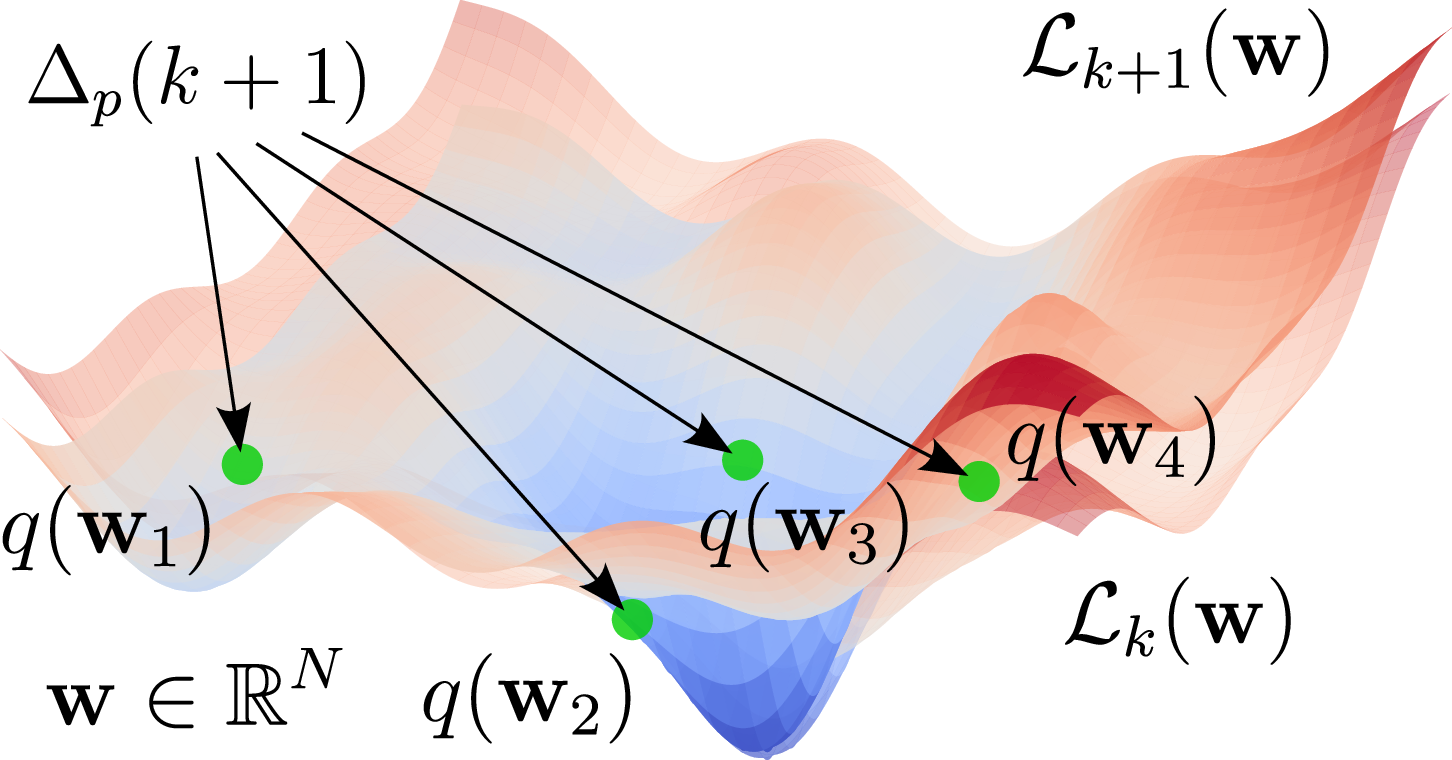
\includegraphics[width=\linewidth]{criterion_general.png}
        \end{figure}
    \end{column}
\end{columns}
\vspace{0.8em}
\begin{enumerate}
    \item Без ограничения общности $\int q(\mathbf{w}) \, d\mathbf{w} = 1$, т.\,е.\ $q(\mathbf{w})$ "--- плотность распределения;
    \item Существующие подходы "--- частные выборы пары~$(p, q)$: одноточечный (Дирак) и среднеквадратичный (гаусс в $\mathbb R^N$);
    \item Локальный интерес $\Rightarrow$ $q(\mathbf{w})$ с массой возле минимума.
\end{enumerate}
\end{frame}

\begin{frame}{Абсолютный одноточечный критерий сходимости}
\begin{columns}[T]
    \begin{column}{0.59\textwidth}
        \hspace*{0.3em}
        \begin{minipage}{\linewidth}
            \begin{equation*}
                \Delta_{1}(k+1) = | \mathcal{L}_{k+1}(\mathbf{w}) - \mathcal{L}_{k}(\mathbf{w}) |,
            \end{equation*}
            где $\mathbf{w} \in \mathcal{U}_{R}(\mathbf{w}_k^*)$ "--- точка из окрестности радиуса $R>0$ минимума $\mathbf{w}_k^{*}$, т.\,е. $p=1$ и $q(\tilde{\mathbf{w}}) = \delta(\tilde{\mathbf{w}} - \mathbf{w})$. Теоретические свойства критерия определяются вектором градиента $\mathbf{g}_{k}(\mathbf{w}) = \nabla_{\mathbf{w}} \mathcal{L}_{k}(\mathbf{w})$ функции потерь и ее матрицей Гессе $\mathbf{H}_{k}(\mathbf{w}) = \nabla_{\mathbf{w}}^2 \mathcal{L}_{k}(\mathbf{w})$.
        \end{minipage}
    \end{column}
    \hspace{0.2em}
    \begin{column}{0.4\textwidth}
        \begin{figure}
            \centering
            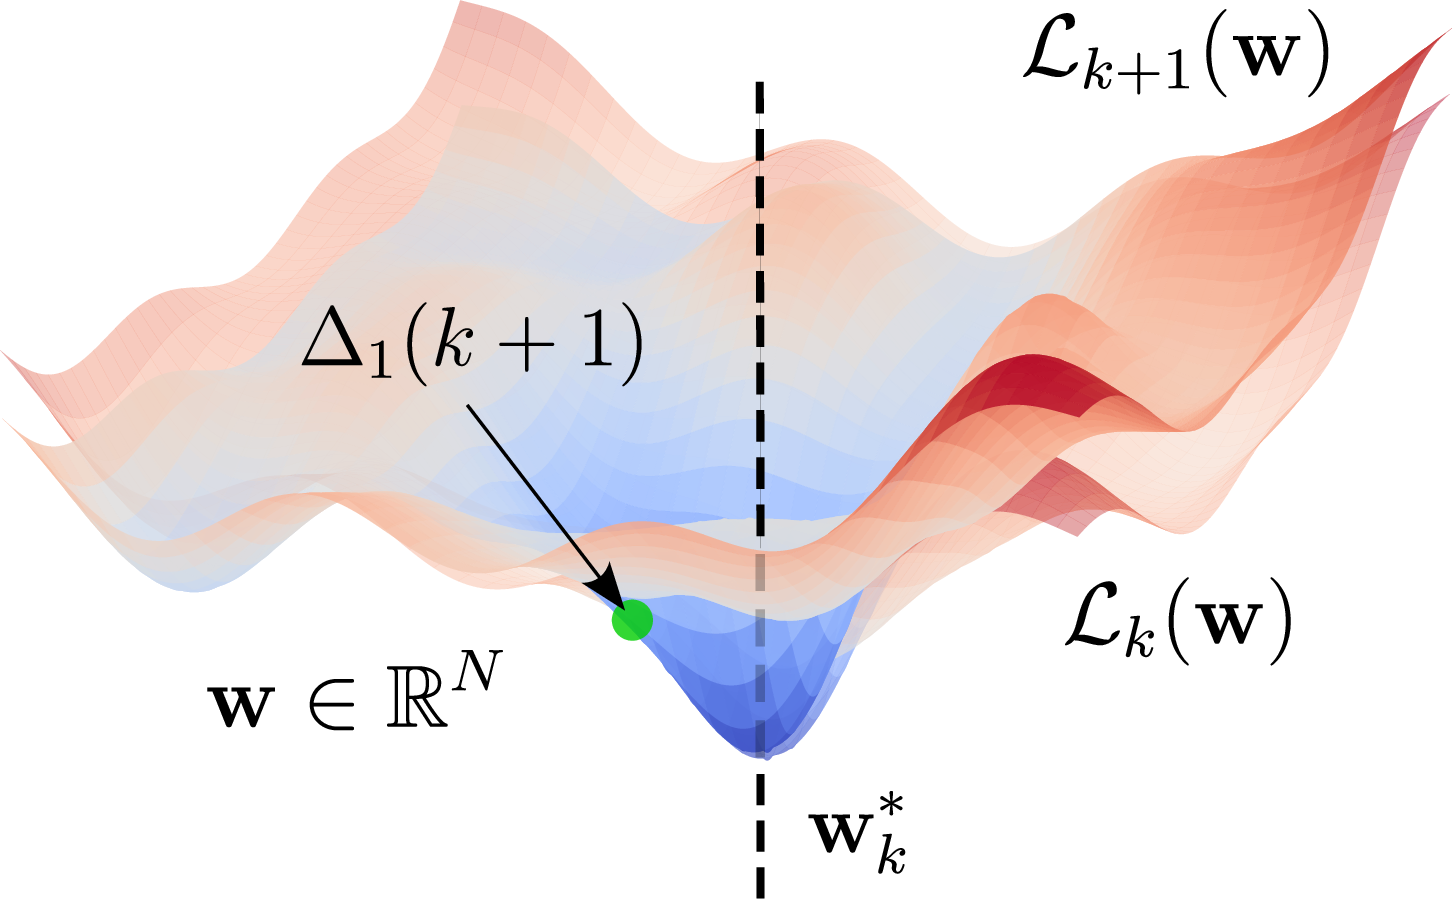
\includegraphics[width=\linewidth]{criterion_abs.png}
        \end{figure}
    \end{column}
\end{columns}
\begin{block}{Теорема (Киселев, 2024)}
    Пусть в $\mathcal{U}_{R}(\mathbf{w}_k^*)$ справедлива квадратичная аппроксимация $\mathcal{L}_{k}(\mathbf{w})$, причем $\| \mathbf{g}_{k+1}(\mathbf{w}_k^*) \|_2 \leqslant M_{\mathbf{g}}$ и для всех $i = 1, \ldots, k+1$ верно $| \ell_{i}(\mathbf{w}_k^*) | \leqslant M_{\ell}$, $\| \mathbf{H}_{i}(\mathbf{w}_k^*) \|_2 \leqslant M_{\mathbf{H}}$, тогда
    \begin{equation*}
        \Delta_{1}(k+1) \leqslant \frac{2 M_{\ell} + M_{\mathbf{g}} R + M_{\mathbf{H}} R^2}{k + 1} = \mathcal{O}(k^{-1}).
    \end{equation*}
\end{block}
\end{frame}

\begin{frame}{Среднеквадратичный критерий сходимости}
\begin{columns}[T]
    \begin{column}{0.57\textwidth}
        \hspace*{0.1em}
        \begin{minipage}{\linewidth}
            \vspace{-0.2em}
            \begin{equation*}
                \Delta_{2}(k+1) = \mathbb{E}_{q(\mathbf{w})} \left[ \big( \mathcal{L}_{k+1}(\mathbf{w}) - \mathcal{L}_{k}(\mathbf{w}) \big)^2 \right],
            \end{equation*}
            \vspace{-1.2em}

            т.\,е. $p=2$, для теоретического анализа удобно выбрать $q(\mathbf{w}) = \mathcal{N}(\mathbf{w}_k^*, \sigma^2 \mathbf{I}_N)$, а на практике базово вычисляется методом Монте"--~Карло через $\mathbf{w}_s \sim q(\mathbf{w})$:
            \vspace{-1.0em}
            \begin{equation*}
                \hat{\Delta}_{2}(k+1) = \frac{1}{S} \sum_{s=1}^{S} \big( \mathcal{L}_{k+1}(\mathbf{w}_s) - \mathcal{L}_{k}(\mathbf{w}_s) \big)^2.
            \end{equation*}
        \end{minipage}
    \end{column}
    \hspace{0.2em}
    \begin{column}{0.4\textwidth}
        \begin{figure}
            \centering
            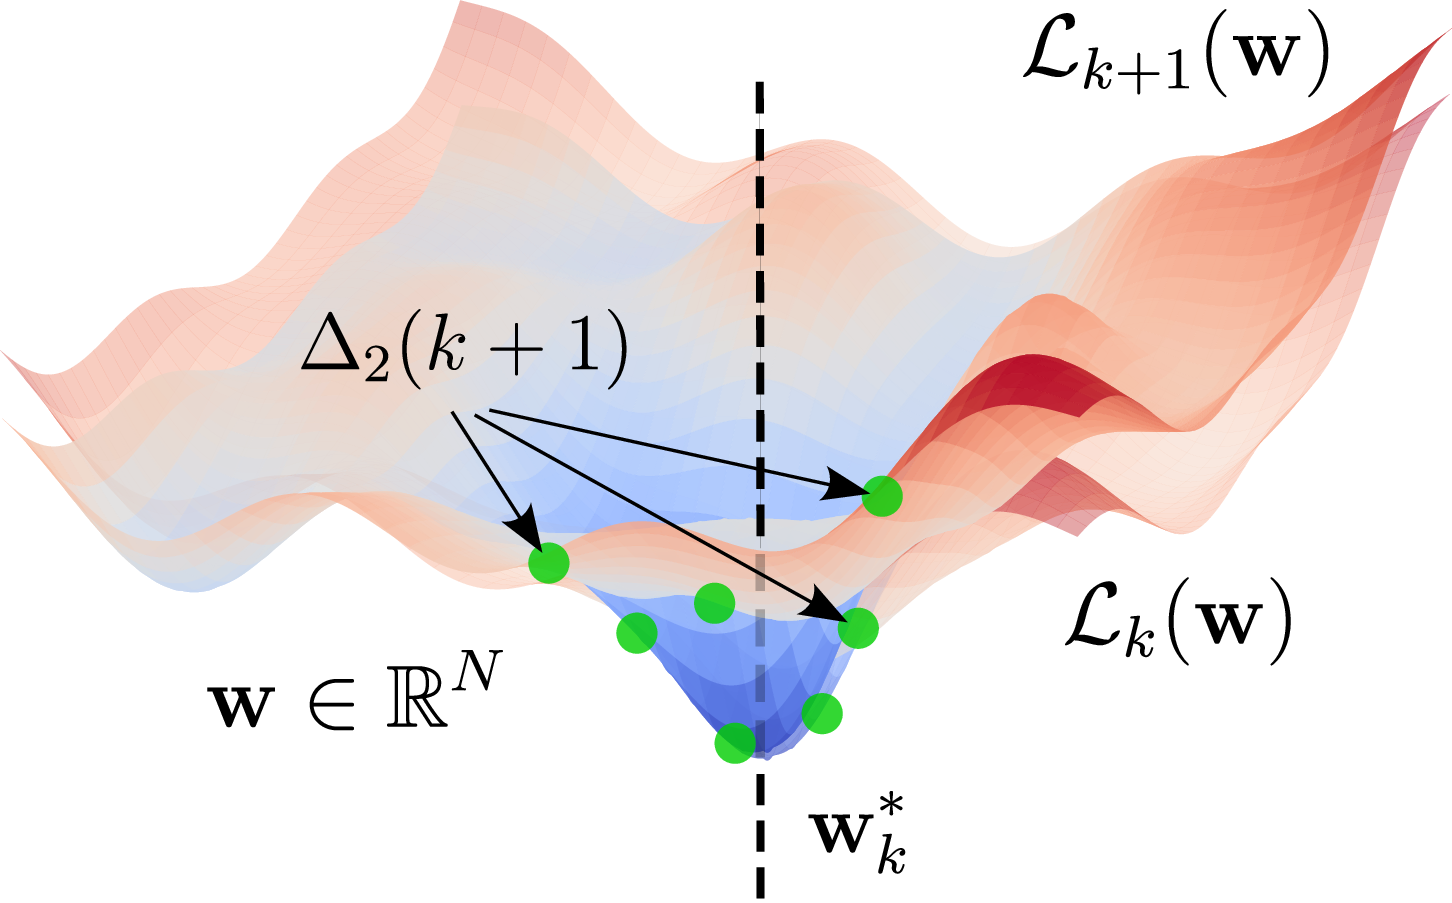
\includegraphics[width=\linewidth]{criterion_squared.png}
        \end{figure}
    \end{column}
\end{columns}
\begin{block}{Теорема (Киселев, 2025)}
    Пусть в $\mathcal{U}_{R}(\mathbf{w}_k^*)$ справедлива квадратичная аппроксимация $\mathcal{L}_{k}(\mathbf{w})$, причем $\| \mathbf{g}_{k+1}(\mathbf{w}_k^*) \|_2 \leqslant M_{\mathbf{g}}$ и для всех $i = 1, \ldots, k+1$ верно $| \ell_{i}(\mathbf{w}_k^*) | \leqslant M_{\ell}$, $\| \mathbf{H}_{i}(\mathbf{w}_k^*) \|_2 \leqslant M_{\mathbf{H}}$, тогда
    \begin{equation*}
        \Delta_{2}(k+1) \leqslant \frac{12 M_{\ell}^2 + 3 \sigma^2 M_{\mathbf{g}}^2 + 3 \sigma^4 \alert{(N^2 + 2N)} M_{\mathbf{H}}}{(k + 1)^2} = \mathcal{O}(k^{-2}).
    \end{equation*}
\end{block}
\end{frame}

\begin{frame}{Среднеквадратичный критерий сходимости в подпространстве наибольшей кривизны}
\begin{columns}[T]
    \begin{column}{0.58\textwidth}
        \hspace*{0.1em}
        \begin{minipage}{\linewidth}
            $\mathbf{H}^{(k)}(\mathbf{w}_k^*) \mathbf{u}_i = \lambda_i^{(k)} \mathbf{u}_i$, $\lambda_{1}^{(k)} \geqslant \ldots \geqslant \lambda_{N}^{(k)}$, $\mathbf{U}_{\alert{D}} = [\mathbf{u}_1, \ldots, \mathbf{u}_{\alert{D}}]$, $\mathcal{S}_{D} = \mathrm{Im}(\mathbf{U}_{\alert{D}})$, тогда критерий с $\mathrm{supp} \ q \subset \mathbf{w}_k^* + \mathcal{S}_{\alert{D}}$:
            \vspace{-0.6em}
            \begin{equation*}
                \Delta_{2}^{(\alert{D})}(k+1) = \mathbb{E}_{q(\mathbf{w})} \left[ \big( \mathcal{L}_{k+1}(\mathbf{w}) - \mathcal{L}_{k}(\mathbf{w}) \big)^2 \right],
            \end{equation*}
            \vspace{-1.8em}
            
            На практике базово вычисляется методом Монте"--~Карло через $\mathbf{w}_s = \mathbf{w}_k^* + \mathbf{U}_{D} \mathbf{z}_s$, где $\mathbf{z}_s \sim \mathcal{N}(\mathbf{0}, \sigma^2 \mathbf{I}_{\alert{D}})$ и $D \ll N$.
        \end{minipage}
    \end{column}
    \hspace{0.2em}
    \begin{column}{0.4\textwidth}
        \begin{figure}
            \centering
            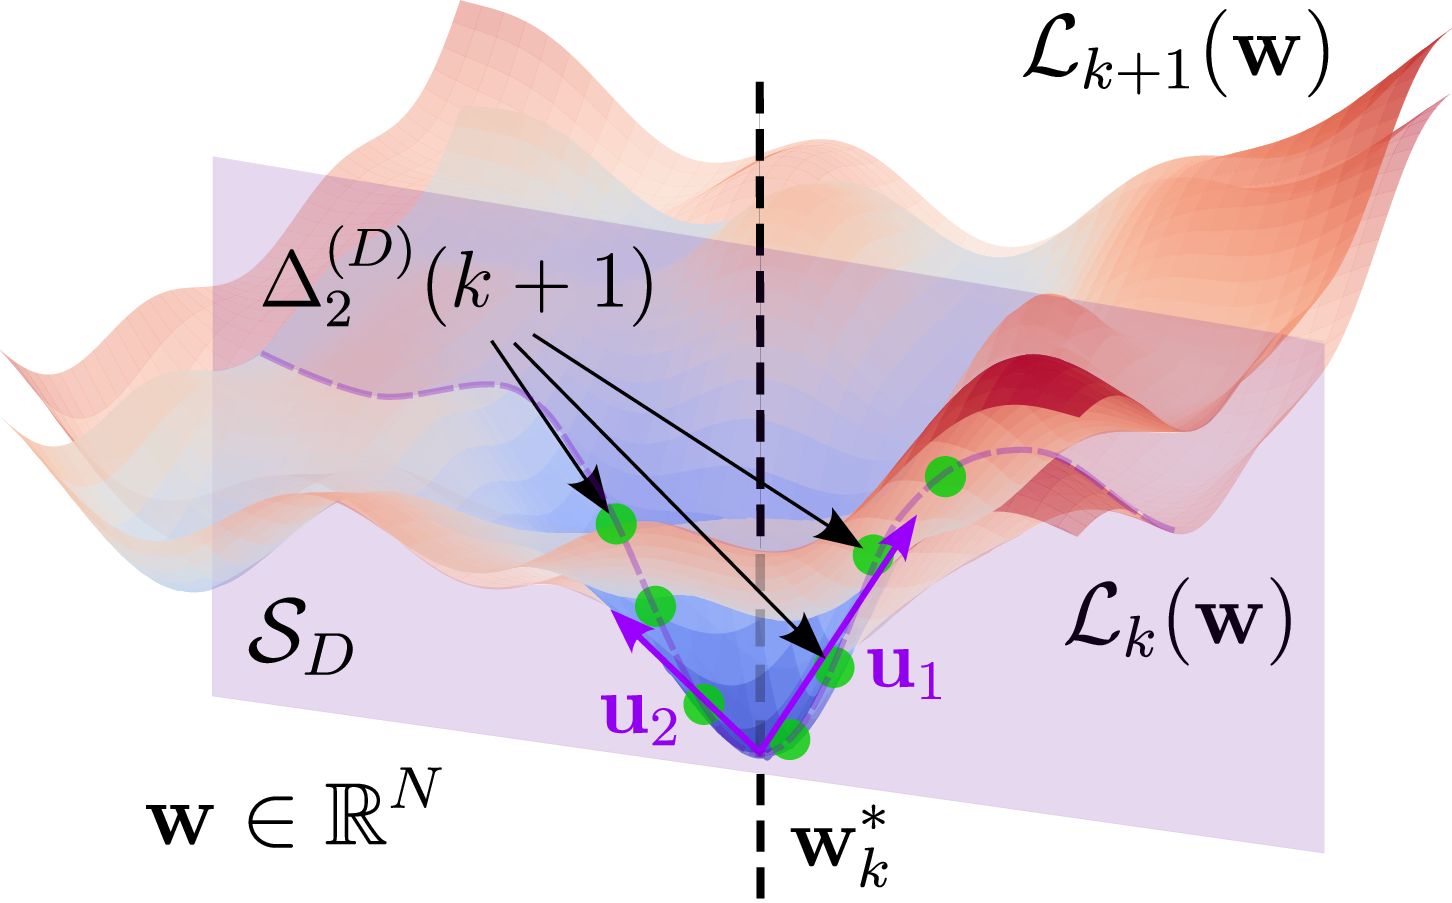
\includegraphics[width=\linewidth]{criterion_squared_subspace.png}
        \end{figure}
    \end{column}
\end{columns}

\begin{block}{Теорема (Киселев, 2026)}
    Пусть в $\mathcal{U}_{R}(\mathbf{w}_k^*)$ справедлива квадратичная аппроксимация $\mathcal{L}_{k}(\mathbf{w})$, причем $\| \mathbf{g}_{k+1}(\mathbf{w}_k^*) \|_2 \leqslant M_{\mathbf{g}}$ и для всех $i = 1, \ldots, k+1$ верно $| \ell_{i}(\mathbf{w}_k^*) | \leqslant M_{\ell}$, $\| \mathbf{H}_{i}(\mathbf{w}_k^*) \|_2 \leqslant M_{\mathbf{H}}$, тогда
    \begin{equation*}
        \Delta_{2}^{(D)}(k+1) \leqslant \frac{12 M_{\ell}^2 + 3 \sigma^2 M_{\mathbf{g}}^2 + 3 \sigma^4 \alert{(D^2 + 2D)} M_{\mathbf{H}}}{(k + 1)^2} = \mathcal{O}(k^{-2}).
    \end{equation*}
\end{block}
\end{frame}

\begin{frame}{Численные методы оценки $\Delta_2^{(D)}$}
    \small
    \begin{block}{Цель}
        % \small
        Численно оценить $\Delta_{2}^{(D)}(k+1) = \mathbb{E}_{q(\mathbf{w})}\!\left[ \big( \mathcal{L}_{k+1}(\mathbf{w}) - \mathcal{L}_{k}(\mathbf{w}) \big)^2 \right]$ при $\mathbf{w} = \mathbf{w}_k^* + \mathbf{U}_{D} \mathbf{z}$, $\mathbf{z} \sim \mathcal{N}(\mathbf{0}, \sigma^2 \mathbf{I}_{D})$. В координатах $\mathbf z$ разность аппроксимируется квадратично: $\mathcal L_{k+1}(\mathbf w) - \mathcal L_k(\mathbf w) \approx a_k + \mathbf c_k^\top \mathbf z + \tfrac12 \mathbf z^\top \mathbf B_k \mathbf z$, $a_k = \mathcal L_{k+1}(\mathbf w_k^*) - \mathcal L_k(\mathbf w_k^*)$, $\mathbf c_k = \mathbf U_D^\top \mathbf g^{(k+1)}$, $\mathbf B_k = \mathbf U_D^\top(\mathbf H^{(k+1)} - \mathbf H^{(k)})\mathbf U_D$.
    \end{block}
    \begin{block}{Методы оценки}
        \begin{enumerate}
        \item \textbf{Монте"--~Карло:} прямое усреднение по $S$ сэмплам \hfill\alert{$\mathcal O\big(S(ND+C_{\mathrm{fwd}})\big)$}
        \vspace{-1.0em}
        \begin{equation*}
            \hat{\Delta}_{2}(k+1) = \dfrac{1}{S} \sum_{s=1}^{S} \big( \mathcal{L}_{k+1}(\mathbf{w}_s) - \mathcal{L}_{k}(\mathbf{w}_s) \big)^2
        \end{equation*}
        \vspace{-1.6em}
        \item \textbf{Квадратичная Монте"--~Карло:} подстановка аппроксимации \hfill\alert{$\mathcal O(SD^2)$}
        \vspace{-1.0em}
        \begin{equation*}
            \hat{\Delta}_{2,\mathrm{quad}}^{(D)}(k+1) = \dfrac{1}{S} \sum_{s=1}^{S} \big( a_k + \mathbf c_k^\top \mathbf z_s + \dfrac12 \mathbf z_s^\top \mathbf B_k \mathbf z_s \big)^2
        \end{equation*}
        \vspace{-1.6em}
        \item \textbf{Замкнутая форма (GM):} аналитическое усреднение по $\mathbf z_s$ \hfill\alert{$\mathcal O(D^2)$}
        \vspace{-1.0em}
        \begin{equation*}
            \hat{\Delta}_{2,\mathrm{GM}}^{(D)}(k+1) = a_k^2 + a_k \sigma^2 \operatorname{Tr}(\mathbf B_k) + \sigma^2 \|\mathbf c_k\|_2^2 + \dfrac{\sigma^4}{4}\big(2\operatorname{Tr}(\mathbf B_k^2) + \operatorname{Tr}(\mathbf B_k)^2\big)
        \end{equation*}
        \end{enumerate}
    \end{block}
\end{frame}

\begin{frame}{Вычислительный эксперимент 1: подпространство наибольшей кривизны и анизотропия ландшафта}
\textbf{Постановка:} классификация MNIST полносвязной сетью, обучаемой методом Adam. Ведущие собственные векторы матрицы Гессе $\mathbf{H}^{(k)}(\mathbf{w}_k^*)$ вычисляются итерационным спектральным методом на произведениях матрицы Гессе на вектор.
\vspace{-1.2em}
\begin{columns}[T]
    \begin{column}{0.4\textwidth}
        \begin{figure}
            \centering
            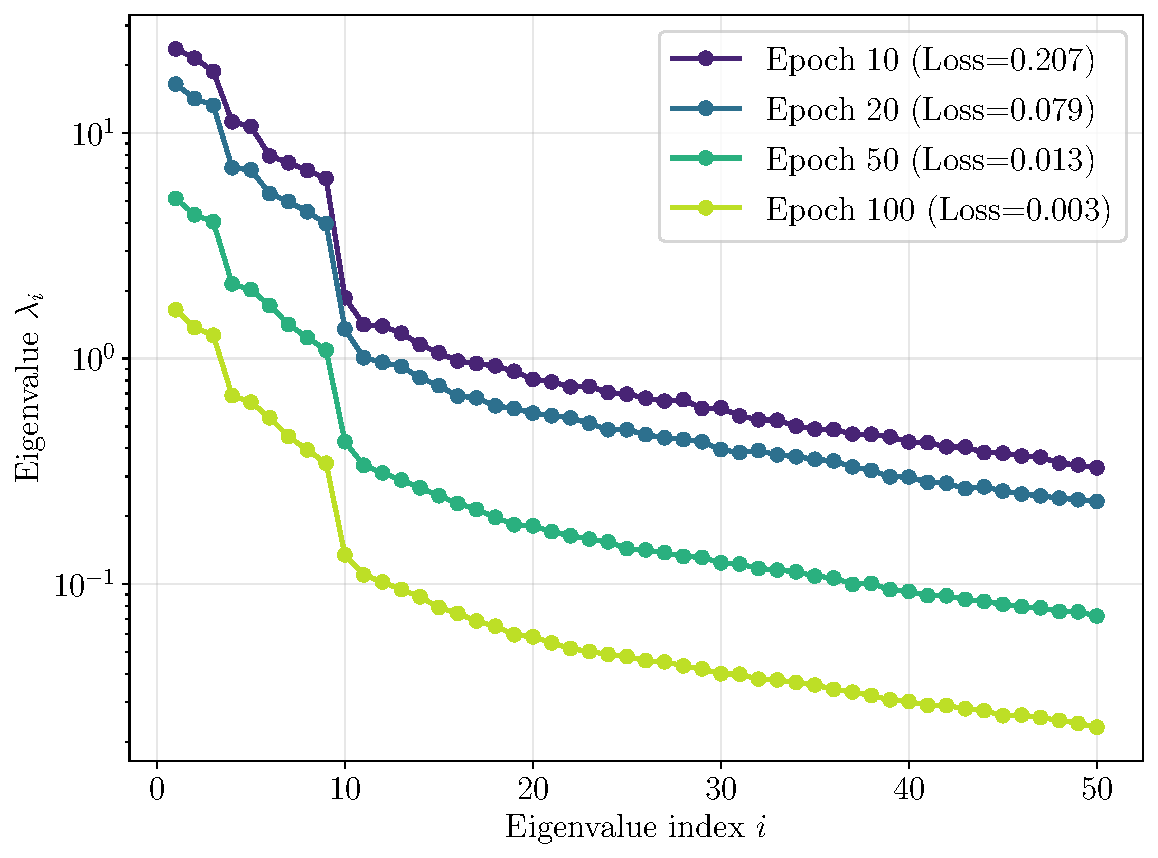
\includegraphics[width=0.9\linewidth]{hessian_spectrum.pdf}
        \end{figure}
    \end{column}
    \begin{column}{0.6\textwidth}
        \begin{figure}
            \centering
            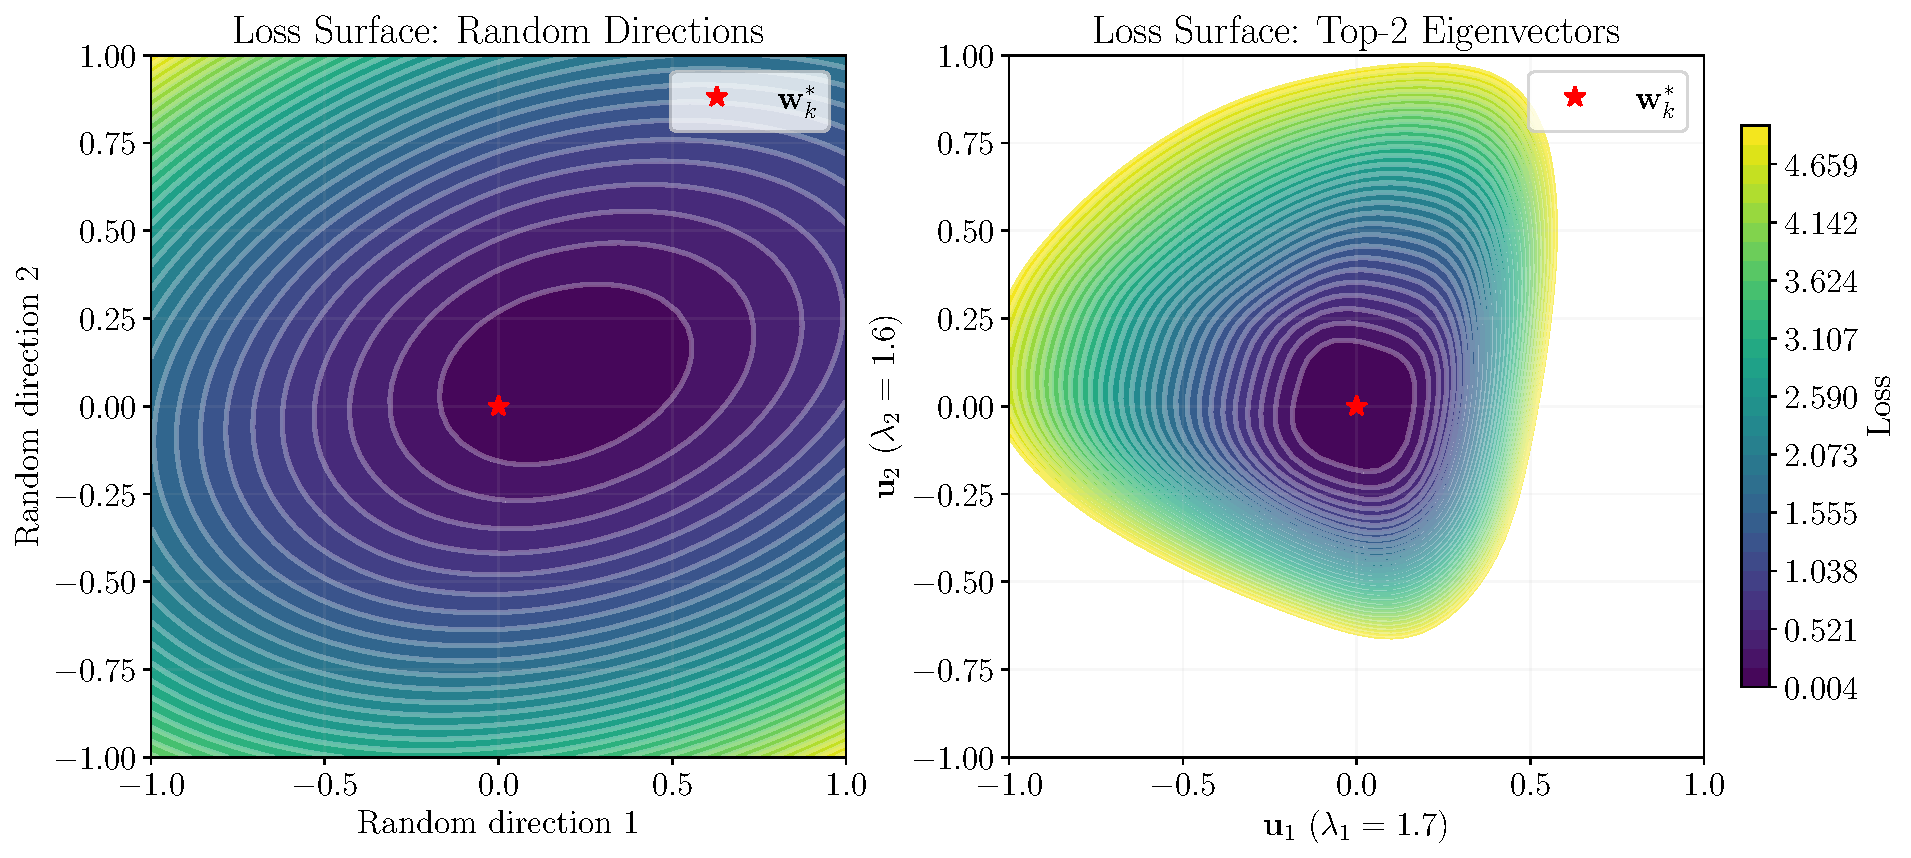
\includegraphics[width=\linewidth]{loss_surface_2d.pdf}
        \end{figure}
    \end{column}
\end{columns}
Собственные значения убывают $\Rightarrow$ \alert{\textbf{локализация кривизны}} в подпространстве небольшой размерности. Двумерные сечения функции потерь вдоль ведущих собственных векторов сильно \alert{\textbf{анизотропны}} в сравнении со случайными направлениями.
\end{frame}

\begin{frame}{Вычислительный эксперимент 2: скорость убывания критериев и подгонка степенного закона}
    Зависимость критериев $\Delta_1(k)$, $\Delta_2(k)$ и $\Delta_2^{(D)}(k)$ от размера обучающей выборки $k$ оценивается методом Монте"--~Карло на сетке $k \in \{100, 150, \ldots, 10^4\}$. К каждой зависимости подгоняется степенной закон $\Delta(k) \sim k^{-\alpha}$.
    
    \begin{columns}
        \begin{column}{0.55\textwidth}
            \begin{figure}
                \centering
                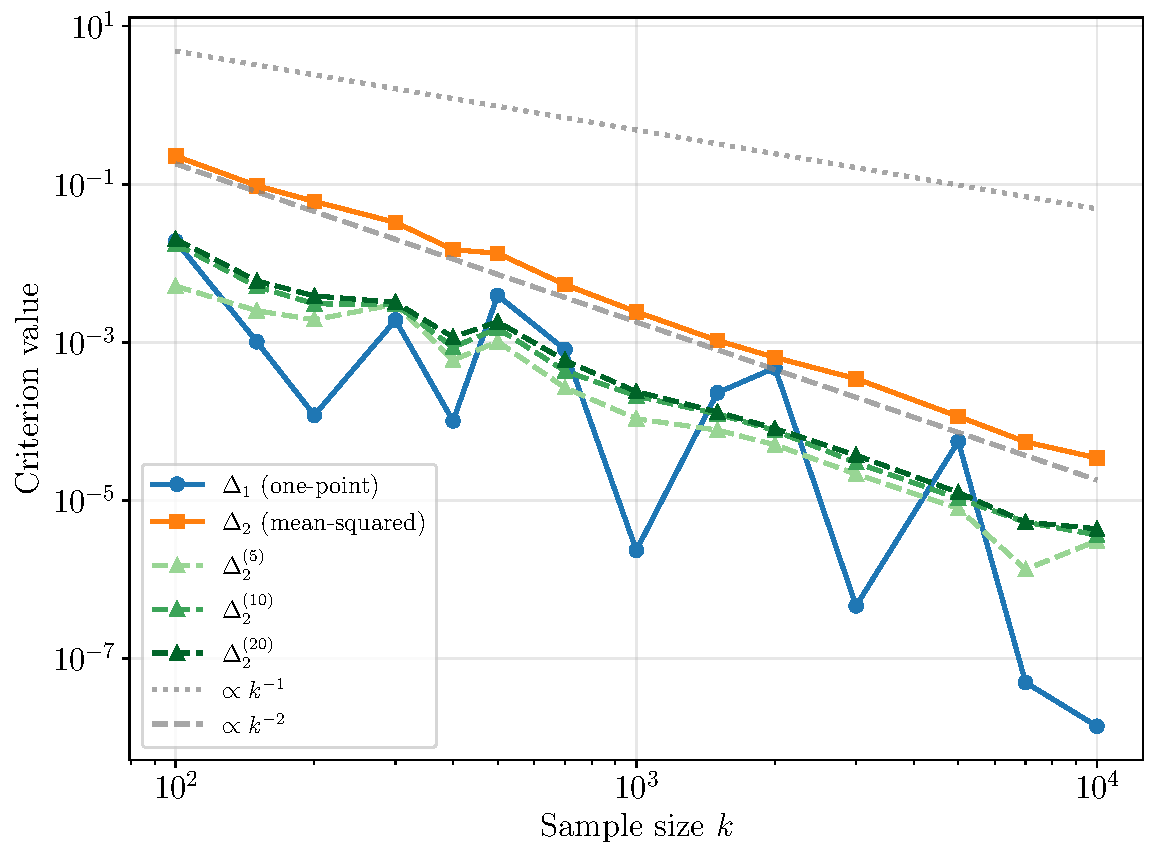
\includegraphics[width=0.75\linewidth]{landscape_convergence.pdf}
            \end{figure}
        \end{column}
        \begin{column}{0.48\textwidth}
            \begin{tabular}{@{}lccc@{}}
                \toprule
                Критерий & $\alpha$ & $R^2$ & Теория \\
                \midrule
                $\Delta_1$ & $2{,}33$ & $0{,}63$ & $1$ \\
                $\Delta_2$ & $1{,}94$ & $1{,}00$ & $2$ \\
                $\Delta_2^{(D=5)}$ & $1{,}80$ & $0{,}96$ & $2$ \\
                $\Delta_2^{(D=10)}$ & $1{,}83$ & $0{,}99$ & $2$ \\
                $\Delta_2^{(D=20)}$ & $1{,}84$ & $0{,}99$ & $2$ \\
                \bottomrule
            \end{tabular}
        \end{column}
    \end{columns}
    
    Численные показатели $\alpha$ для $\Delta_2$ и $\Delta_2^{(D)}$ согласуются с теоретическими.
\end{frame}

\begin{frame}{Выносится на защиту}
    \footnotesize
    \begin{enumerate}
        \item Предложен унифицированный критерий $p$-сходимости $\Delta_p$ с функцией предпочтения в пространстве параметров. Критерий охватывает одноточечную и интегральные постановки стабилизации ландшафта функции потерь.
        \item Введен среднеквадратичный критерий $\Delta_2^{(D)}$ в подпространстве ведущих собственных векторов Гессе. Доказаны теоремы об экстремальности этого подпространства и разработаны численные методы оценки критерия.
        \item Эмпирически исследована сходимость критерия $\Delta_2^{(D)}$ при увеличении размера выборки. На основе оценок скорости убывания критерия предложен метод определения достаточного объема обучающих данных.
    \end{enumerate}
    {\usebeamercolor[fg]{block title} Публикации в рецензируемых научных журналах (ВАК, Scopus)}\\
    \begin{enumerate}
        \item \textit{\textbf{Kiselev N.}, Meshkov V., Grabovoy A.} Robust Convergence of Loss Landscapes through Distributional Averaging~// \textit{Proceedings of the ISP RAS}, 2025.
        \item \textit{Meshkov V., \textbf{Kiselev N.}, Grabovoy A.} ConvNets Landscape Convergence: Hessian-Based Analysis of Matricized Networks~// \textit{Ivannikov Ispras Open Conference (ISPRAS) -- IEEE}, 2024.
        \item \textit{\textbf{Kiselev N.}, Grabovoy A.} Unraveling the Hessian: A Key to Smooth Convergence in Loss Function Landscapes~// \textit{Doklady Mathematics}, 2024.
    \end{enumerate}
\end{frame}

\end{document} 